% hello.tex - Our first LaTeX example!

\documentclass{article}
\usepackage[dvipsnames]{xcolor}
\usepackage{pgf,tikz,pgfplots,graphicx}
\usepackage{wrapfig}
\usepackage{lipsum}
\usepackage{multicol}
\usepackage{amsmath,amsfonts}
\pgfplotsset{compat=1.3}
\usepackage{mathrsfs}
\usepackage{mathtools}
\usepackage{caption}
\usepackage{subcaption}
\usepackage{comment}
\usepackage{enumitem}

\setlength{\columnseprule}{0.8pt}
\def\columnseprulecolor{\color{black}}

\newcommand{\redbox}[1]{%
     \fcolorbox{red}{white}{
     \parbox{\textwidth}{%
        #1
    }%
    }
}
\newcommand\reddashedbox[1]{
\tikz [baseline=(boxed word.base)] \node (boxed word) [draw=red, rectangle, dashed, line cap=round] {#1};
}
\newcommand\redboxlimited[1]{
\tikz [baseline=(boxed word.base)] \node (boxed word) [draw=red, rectangle,  line cap=round] {#1};
}
\newcommand{\exampleblue}[1]{
    \textcolor{RoyalBlue}{#1}
}
\newcommand{\emphexampleorange}[1]{
    \textcolor{Peach}{#1}
}
\newcommand*\theoremsquare[1]{\tikz[baseline=(char.base)]{
            \node[shape=rectangle,draw,inner sep=2pt] (char) {\footnotesize #1};}}
\newcommand*\circled[1]{\tikz[baseline=(char.base)]{
            \node[shape=circle,draw,inner sep=0.7pt] (char) {#1};}}
\usetikzlibrary{arrows}

\begin{document}

\title{Calculus Notes}
\author{Jack Gong\\
Pinetree Secondary\\
  \texttt{haotiangong@hotmail.com}}
\date{\today}
\maketitle
\newpage
\tableofcontents
\newpage



\section{Intro}

\subsection{Ideas about Sets}

\redbox{Definition of a set: a collection of distinct objects. These objects are called the elements of the set.}

We use $\{\}$ to enclose elements of the set. Two sets are the same if they contain the same objects. The size, or cardinality of a set is the number of (distinct) elements in that set. It may be infinite.

\medskip
Sets can be ``arbitrarily declared" without following the rule of distinct elements. For example, $$ \{ 1,1,2,2,3,3,4,4,5,5\} = \{ 1,2,3,4,5\}$$

\subsection{Sets We Use Frequently}

\begin{itemize}
\item $\mathbb{N}=\{ 1,2,3,4,5,...\}$
\item $\mathbb{Z}=\{-2,-1,0,1,2,...\}$
\item $\mathbb{Q} $ How do we define rational numbers?
\item $\mathbb{R} $ What about real numbers?
\end{itemize}

\noindent \exampleblue{Trying to define rationals}

1st attempt: Set of all numbers that can be expressed in the form $\frac{a}{b}$ , where $a$ and $b$ are integers and $b \neq 0$.

But how do we define ``numbers"?

2nd attempt (to avoid explaning the definition):  Define S to be the set of all pairs of integers $(a,b)$, where $b \neq 0$; and declare that the pair $(a,b)$ is the same as the pair $(a', b')$ if $ab'  = a'b$.

$\mathbb{Q}$ is the set of results of $\frac{a}{b}$.

\subsection{More definitions}

\hspace{4mm} If S \& T are sets, their union is the set consisting of all elements that are elements of S or are elements of T, or both. We write this as:
\redboxlimited{$S \cup T$.}
\medskip

Different notation: $$S\cup T = {x: x \in S \text{ or }  x \in T} $$

If S and T are sets, the intersection of S and T is the set consisting of all elements that are in S and T.

\medskip
\redbox{ $$S \cap T = {x: x\in S \text{ and } x\in T}$$}

If S and T are sets and every element of S is also an element of T, then we say T contains S and write this as

\medskip
\redbox{ $$S \subset T \text{ or } T \supset S$$}

If S and T are sets, we also define the set difference operation:

\medskip
\redbox{$$S \setminus T = { x: x\in S \text{ and } x\notin T}$$}

\noindent \exampleblue{How do we express the elements in $\{ x: x\in S \text{ or } x\in T, \text{ but not both?} \} $}
\medskip

We can express it as $ (S\setminus T) \cup (T\setminus S)$ or $(S\cup T) \setminus (S\cap T)$. (It can also be expressed as $S \bigtriangleup T$)

How do we proove that these sets actually equal to each other? We can proove that $ \subset \text{ and } \supset $ goes both ways. If a set includes the other and the other includes the set, they are equal.
\medskip

Empty (null) set: $\{\} = \emptyset$

If $S$ and $T$ are sets and $S \cap T = \emptyset $, we say $S$ and $T$ are \textbf{disjoint}.

\subsection{Properties of Reals}

Defining the reals is a tedious task. Rather than defining the real numbers, we will describe some of their properties.

\begin{itemize}
  \item $\mathbb{R}$ is a set. It contains the national numbers.
  \item They can be added and subtracted.
  \item They can be multiplied and divided.
  \item The real numbers arre ordered. If $x,y \in \mathbb{R}$, then either $x<y$, $x=y$, or $x>y$.
  \item Product of 2 positives or negatives is positive; product of positive and negative is negative.
  \item The $\mathbb{R}s$ follow the \textbf{Least upper bound property}.
\end{itemize}

\subsection{The Least Upper Bound Property}

\redbox{If $S \subset \mathbb{R}$ ,  a real number $\mathbb{R}$ is called an upper bound for $S$ if:
        $$ \text{ For all }(\forall) y \in S, \text{ we have } y\leq x.$$}

\noindent\exampleblue{Is the upper bound of $T = \{ x \in \mathbb{R}, x<0 \}$ in T? \\ Prove: For every $x \in T$, there exists a number $y \in T$ with $y>x$.}
\medskip

Proof: Let $y = \frac{x}{2}$. We need to show ( $y\in T$ and $y>x$ )

\circled{1} Since $\frac{1}{2}$ is positive, $y = \frac{1}{2}x$ has the same sign as $x$.\\
Since $x<0$, we conclude $y<0$. Hence $y\in T$.

\circled{2} Since $x<0$, and $0<\frac{1}{2}<1$, we have $y = \frac{x}{2} >x$.

We conclude if $x\in T$, then $x$ is not an upper bound for T.

\reddashedbox{Some sets $S\subset \mathbb{R}$ have an upper bound, some don't.}

If $S \subset \mathbb{R}$ has an upper bound, we say it is \textbf{bounded above}; oherwise it is not bounded above.
\medskip

Let $S \subset \mathbb{R}$. A number $x \in \mathbb{R}$ is called a least upper bound for $S$ if
\begin{enumerate}
  \item $x$ is an upper bound for $S$.
  \item If $z \in \mathbb{R}, z<x$, then $z$ is not an upper bound for $S$.
\end{enumerate}

\redbox{Least upper bound property: if $S\subset \mathbb{R}$ and $S$ is bounded above, then $S$ has a least upper bound.}

\subsubsection{Least Upper Bound and $\mathbb{Q}$}
\emphexampleorange{How do we show the least upper bound prop. isn't true for all $\mathbb{Q}$s?}

\medskip
Thought: construct a set whose least upper bound is a real number.
\medskip

Let $S = \{ x\in \mathbb{Q}, x>0, \text{ and } x^2 <2\}$

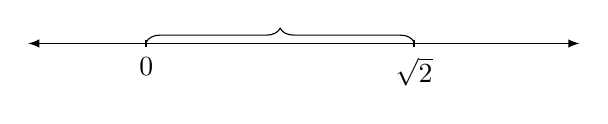
\begin{tikzpicture}
\draw[latex-latex] (-3.5,0) -- (3.5,0) ; %edit here for the axis
\foreach \x/\y in {-2/0, 1.4/\sqrt{2}}
 \draw[thick] (\x,0.05) -- (\x,-0.05) node[below]{$\y$};
\draw[decorate,decoration={brace,amplitude=5pt,raise=0.5pt},yshift=0pt] (-2,0) -- (1.4,0);
\end{tikzpicture}

We will show: \begin{enumerate}
  \item S is bounded above. Indeed, if $x\in \mathbb{Q}, x^2>2,$ then x is an upper bound and $x>0$.
  \item If $y\in \mathbb{Q}$ is an upper bound for $S$, then there exists $z\in \mathbb{Q}$, with $z<y$ and $z$ is also an upper bound.
\end{enumerate}

\subsection{Proof by Contradiction}
The goal is to prove some mathematical statement.
\begin{enumerate}
  \item Suppose the statement is false.
  \item Using the assumption that the statement is false, and its relevant deductions,
  \item arrive at the conclusion it is clearly false.
  \item Conclude the original statement is false.
\end{enumerate}

\subsection{Open and Closed Intervals}
We can think of real numbers as points on a number line.

\begin{center}
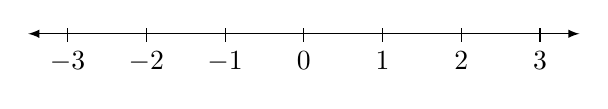
\begin{tikzpicture}
\draw[latex-latex] (-3.5,0) -- (3.5,0) ; %edit here for the axis
\foreach \x in  {-3,-2,-1,0,1,2,3} % edit here for the vertical lines
\draw[shift={(\x,0)},color=black] (0pt,2pt) -- (0pt,-2pt);
\foreach \x in {-3,-2,-1,0,1,2,3} % edit here for the numbers
\draw[shift={(\x,0)},color=black] (0pt,0pt) -- (0pt,-3pt) node[below]
{$\x$};
\end{tikzpicture}
\end{center}

An \textbf{open interval} is a subset of $\mathbb{R}$ of one of the following forms:

\begin{enumerate}
  \item  $ \begin{cases}
    {x \in \mathbb{R}, x>a \text{ and } x<b}, \text{, where} a,b \in \mathbb{R}, a<b\\
    {x \in \mathbb{R}: a<x<b}\\
    (a,b)
  \end{cases} $\\
  We have finite length open intervals with length $b-a$.
  \item   $ \begin{cases}
    {x \in \mathbb{R}: x>a}, \text{, where } a\in \mathbb{R}\\
    (a,\infty)
  \end{cases} $
  \item   $ \begin{cases}
    {x \in \mathbb{R}: x<b}, \text{, where } b\in \mathbb{R}\\
    (-\infty,b)
  \end{cases} $
  \item   $ \begin{cases}
    {x \in \mathbb{R}}\\
    (-\infty, \infty)
  \end{cases}$
\end{enumerate}

A \textbf{closed interval} is a subset of $\mathbb{R}$ of one of the following forms:
\begin{enumerate}
  \item  $ \begin{cases}
          {x\in \mathbb{R}: a\leq x\leq b}\;\; a,b \in \mathbb{R}, a<b\\
          [a,b]
         \end{cases}$\\
  \item $ \begin{cases}
          {x\in \mathbb{R}}: a\leq x\\
          [a,\infty]
         \end{cases}$
  \item $ \begin{cases}
         {x\in \mathbb{R}}: x\leq b\\
         [-\infty,b]
        \end{cases}$
  \item $\mathbb{R}$
\end{enumerate}

\exampleblue{What about the sets $(a,b]$ or $[a,b)$?}
``Half-open" interval.

\subsection{Function Definitions}

\redbox{A function is a rule $f$ that assigns to each element $x$ of a set $D$, called the domain, a unique element $f(x)$ of a set $S$, called the co-domain.}

The domain and co-domain can be the same set.

We write:
\medskip

\noindent\redbox{$$x\in D, f(x) \in S \text{, and } f:D \rightarrow S$$}

Example: $D: \{ 1,2,3,4 \},\; S\subset\mathbb{R}$, and $f$ is given by $f(1) = 1, f(2) = 1, f(3) = \pi, f(4) = -3$

\begin{itemize}
  \item $D = \mathbb{R}, f(x) = 0, f(x) = x, f(x) = x^2+x+1$ - \textbf{Polynomials}
  \item $D = \mathbb{R}, f(x) = sinx, f(x) = cosx, f(x) = sin(2x)$ - \textbf{Trignometric functions}
  \item $D = \mathbb{R}, f(x) = e^x, f(x) = e^2x$ - \textbf{Exponential functions}
  \item $D = (0, \infty), f(x) = logx, f(x) = \frac{1}{2}logx$ - \textbf{Logarithmic functions}
\end{itemize}

We choose to study these special cases of functions because most mathematical aspects of the natural word are reflected by them.

\medskip
\exampleblue{Domain convention}: If the domain of a function isn't specified, we assume the domain is the largest subset of $\mathbb{R}$ for which $f(x)$ ``makes sense"  as a real number. We will write this as $D(f)$ or $D$ of $f$.

ex. $f(x) = x^2 +2, D(f) = \mathbb{R}$\\
\hspace*{4mm}$f(x) = log(x), D(f) = (0, \infty)$\\
\hspace*{4mm}$f(x) = log|x|, D(f) = (-\infty, 0) \cup (0, \infty)$.

\medskip
\exampleblue{*} Domains including the complex number set is hard to define since defining a domain in one interval can affect numbers in other intervals.

\bigskip
If $f$ is a funtion, the \textbf{range} of $f$ is the set \reddashedbox{$\{ f(x): x\in D(f)\}$.} We write this as $R(f)$.


ex. $f(x) = sinx\;\;\; D(f): \mathbb{R}\;\;\; R(f): [-1,1] \;\;\; Codomain: \mathbb{R}$

\subsubsection{Graphical Representation}

\redbox{If $f$ is a function, the \textit{graph} of $f$ is the set of ordered pairs $\{ (x,f(x))$: $x\in D(f) \}$. This is a subset of the x-y plane $\{(x,y): x,y \in \mathbb{R}\} = R^2$.}

\begin{figure}[h]
\centering
\begin{subfigure}{.5\textwidth}
  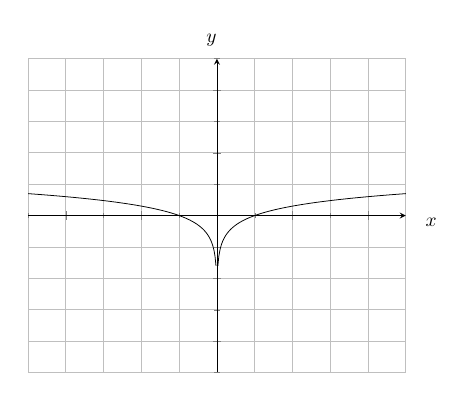
\begin{tikzpicture}[scale = 0.7]
  \begin{axis}[grid=both,ymin=-5,ymax=5,xmax=5,xmin=-5,xticklabel=\empty,yticklabel=\empty,
                 minor tick num=1,axis lines = middle,xlabel=$x$,ylabel=$y$,label style =
                 {at={(ticklabel cs:1.1)}}]
  \addplot[domain = 0:5, samples = 201, color = black]
  {log10(x)};
  \addplot[domain = -5:0, samples = 201, color = black]
  {log10(-x)};
  \end{axis}
  \end{tikzpicture}
  \caption{$f(x)=log|x|$}
\end{subfigure}
\begin{subfigure}{.4\textwidth}
  \centering
  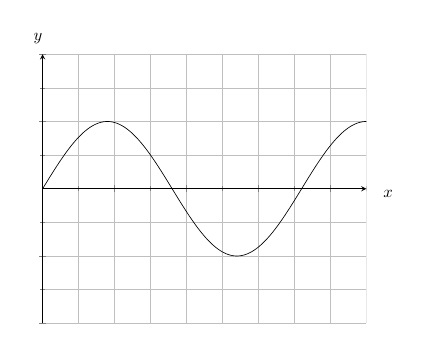
\begin{tikzpicture}[scale = 0.6]

  \begin{axis}[grid=both,ymin=-2,ymax=2,xmax=450,xmin=0,xticklabel=\empty,yticklabel=\empty,
                 minor tick num=1,axis lines = middle,xlabel=$x$,ylabel=$y$,label style =
                 {at={(ticklabel cs:1.1)}}]
  \addplot[domain = 0:450, samples = 401, color = black]
  {sin(x)};
  \end{axis}
  \end{tikzpicture}
  \caption{$f(x)=sinx$}
\end{subfigure}%
\end{figure}

For every subset of the plane(curve), is there a function that yields that subset?

No. Consider the \textbf{vertical line test}. A subset $T\subset \mathbb{R}$ is the graph of a function \underline{if and only if} every vertical line in the xy plane intersects $T$ at most once.

\medskip
\exampleblue{Consider} $\begin{cases}
1,            & \text{if } x\in \mathbb{Q}\\
0,           & \text{if } x \in \mathbb{R} \setminus \mathbb{Q}
\end{cases}$ Is this a function?

\subsection{Injectivity and Surjectivity}
\redbox{A function $f$ is called \textbf{one-to-one} or \textbf{injective} if whenever $$x\neq y, f(x)\neq f(y)$$ Equivelantly, for all $x,y \in D(f)$, $x=y$ if and only if $f(x) = f(y)$.}

\exampleblue{Ex. $f(x) = 2x+1$ injective?}

Yes. Proof: let $x,y$ be in the domain of $f(x)$ and suppose $f(x) = f(y)$. We need to proove $x=y$.

\begin{align*}
  f(x) & = f(y)\\
  2x +1 &= 2y+1\\
  2x &= 2y\\
  x &= y
\end{align*}

\textit{Horizontal Line Test}: A function $f$ is one-to-one if and only if every horizontal line in the xy plane intersects the graph of $f$ in at most one point.

\exampleblue{Ex. $f(x) = x^2 + 1, D = [0,\infty)$ is this one-to-one?}

Proof by contradiction: suppose $f$ is not one-to-one. There exists real numbers $x,y \in D$ so that $x\neq y$, but $f(x) = f(y)$.

\underline{Without loss of generality}, we can assume $x<y$. This implies $x^2 \leq x \cdot y < y \cdot y = y^2$. This is because $x\in [0, \infty)$ implies $x\geq 0$, $y>x$ implies $y>0$, hence $x\cdot y < y \cdot y$, and it follows from $x \geq 0$.

Since $x^2 < y^2$, we have $x^2+1 < y^2 +1$, $f(x) < f(y)$, but this contradicts assumption.

\redbox{A function $f: D \rightarrow S$ is called \textbf{onto} or \textbf{subjective} if we let $R(f) = S$, and for every $y \in S$, there exists $x\in D$ such that $f(x)=y$.
$$ \forall y \in S, \exists\; x\in D\; s.t. \; f(x) = y$$}.

If a function is \textbf{both} one-to-one and onto, we say it is ``one-to-one and onto", or ``bijective".

For every $y\in S$, there exists a unique $x\in D$ such that $f(x) = y$.

$$ \forall y\in S, \; \exists!\: x\in D \; s.t. f(x) = y$$

\subsection{Function interactions}
If $f$ and $g$ are functions, with the domains $D(f)$ and $D(g)$ respectively, then we can define the functions $f+g$, $f-g$, and $f\cdot g$ in obvious ways.

The domain of each of these new functions is \redboxlimited{$D(f)\cap D(g)$}.\\
ex. $f(x) = x^2$ and $g(x) = 1/x$.  $f\cdot g(x) = x$ with Domain $D= \mathbb{R} / {0}$.

\bigskip
We can also define $(f/g)x = \frac{f(x)}{g(x)}$
\begin{align*}
  D(f/g) &= (D(f)\cap D(g)) \setminus \{ x\in D(g), g(x) = 0\}\\
         &= \{ x = D(f) \cap D(g):  g(x) \neq 0\}
\end{align*}

If $f$ and $g$ are functions, we define the compositions \redboxlimited{$ f \circ g = f(g(x))$}. We first apply $g$ then apply $f$.

$$D(f\circ g) = \{ x\in D(g): g(x) \in D(f)\}$$

ex. $g(x) = 1/x$  $f(x) = 1/x$ \\
\hspace*{4mm} $f\circ g(x) = x$ if $x\neq 0$.

\subsection{Triangle inequality}

$$|x+y| \leq |x| + |y|$$
$$||x| - |y|| \leq |x - y|$$

\subsection{Polynomial}
\redbox{
   A \textbf{polynomial} is a function of the form $$f(x) = a_n x^n + a_{n-1} x^{n-1} + ... + a_1 x + a_0$$
   where $a_n ... a_0$ are real numbers, and $a_n \neq 0$.\\

   We define the degree of $f$ to be $n$.
}
\medskip

   \textit{What about $f(x) = 0$?}\\
    Additionally, we say the function $f(x) = 0$ is also a polynomial, and we define its degree to be $-1$.


\subsection{Rational Function}
\redbox{
   A \textbf{rational function} is a function of the form $$f(x) = \frac{P(x)}{Q(x)}$$
   where $P$ and $Q$ are polynomials, and $Q$ is not the zero polynomial.\\

   Every polynomial is a rational function.
}

Ex. $f(x) = \frac{x^2 + 1}{2x + 4}, D(f) = \mathbb{R} \setminus \{ 2 \}$.

\section{Limits}

\subsection{Definition}

Let $f$ be a function, let $a\in \mathbb{R}$, and let $L\in \mathbb{R}$. We Say:\\
\medskip
\redbox{$$ \lim_{x\rightarrow a} f(x) = L $$}\\
If the following holds:\\
\bigskip
\redbox{

  \noindent \textcolor{red}{\theoremsquare{1}} There exists a number $t>0$ so that
  $$ \{ x\in \mathbb{R}: 0<|x-a|<t \} \subset D(f)$$

  \begin{center}
  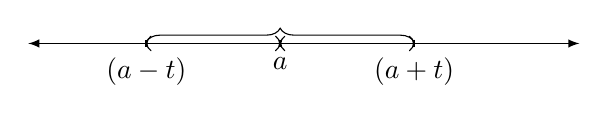
\begin{tikzpicture}

  \draw[latex-latex] (-3.5,0) -- (3.5,0) ; %edit here for the axis
  \foreach \x/\y in {-2/(a-t), -0.3/a, 1.4/(a+t)}
   \draw[thick] (\x,0.05) -- (\x,-0.05) node[below]{$\y$};
  \draw[decorate,decoration={brace,amplitude=5pt,raise=0.5pt},yshift=0pt] (-2,0) -- (1.4,0);
  \draw[(-)] (-2,0) -- (-0.3,0);
  \draw[(-)] (-0.3,0) -- (1.4,0);
  \end{tikzpicture}
  \end{center}

  *$a$ doesn't have to be defined.
}
\medskip
\redbox{
    \textcolor{red}{\theoremsquare{2}} For every real number $\epsilon>0$, there exists a real number $\delta>0$ so that the following is true: For every real number $x$ satisfying the inequality $0<|x-a|<\delta$, we have $f(x) - L <\epsilon$.\\
    $$ \forall \epsilon > 0, \exists\: \delta>0 \text{ s.t. } \forall x \in \mathbb{R} \text{with } 0<|x-a|<\delta, \text{ we have } |f(x) - L | < \epsilon$$
}

\bigskip\bigskip
\noindent\exampleblue{Prove $\lim_{x\rightarrow 3} 2x = 6$.}

\noindent \circled{1} Find a $t>0$ so that: $$\{ x\in \mathbb{R}: 0 <|x-3|<t\} \subset D(f)$$ Any $t>0$ works.\\
\circled{2} Let $\epsilon > 0$, set $\delta = \epsilon/2$\\
Let $x\in \mathbb{R}$ with $0<|x-3|<\delta$.\\
Then $|2x-6| = |2(x-3)| = 2|x-3| < 2\delta = \epsilon = \epsilon.$
\medskip

\noindent\exampleblue{Prove $\lim_{x\rightarrow 4} x^2 = 16$.}\\
Since $D(f) = \mathbb{R}$, the domain requirement is satisfied.\\
Let $\epsilon > 0$, select $\delta = $ min($\epsilon/9, 1$).\\
Let $x\in \mathbb{R}$ with
$$0<|x-4|<\delta$$
$|f(x)-L| = |x^2-16| = |(x-4)(x+4)| = |x+4||x-4|$
\begin{align*}
  |x+4||x-4| &< |x+4| \delta\\
             &\leq (|x|+4) \delta \text{  We specified that $\delta<=1$, then $|x|+4<=5$}\\
             &\leq (5+4)\delta\\
             &= 9\delta \leq \epsilon
\end{align*}
\medskip

\noindent\exampleblue{Prove $\lim_{x\rightarrow 0} 2x\sin(1/x) = 0$}\\
Since $D(f) = \mathbb{R} \setminus {0}$, we can select $t = 1$, and $(-1,0) \cup (0,1) \subset D(f)$.\\
Let $\epsilon >0$, select $\delta = \epsilon/2$\\
Let $x\in \mathbb{R}$ with $0<|x-0|<\delta$.\\
\begin{align*}
   |f(x)-L|  & = |2x \cdot \sin(1/x) - 0|\\
             & = |2x \cdot \sin(1/x)|\\
             &= 2|x||\sin(1/x)|  \;\;\text{   Since  } 0\leq |\sin(1/x)| < 1\\
             &\leq 2|x| = \epsilon
\end{align*}

\subsubsection{Negating statements involving quantifiers}
Every well crafted mathematical statement is either true or false. If $S$ is a statement, either $S$ is true, or $S$ is false (*which is equivalent to ``$S$ is false" is true)

\begin{multicols}{2}
$\forall x\in \mathbb{R}, x^2\geq 0$ is true.

\columnbreak
$\exists x\in \mathbb{R},$ s.t. $x^2<0$.\\
\hspace*{4mm}($\forall x\in \mathbb{R}, x^2\geq 0$ is false.)

\end{multicols}

\noindent\redbox{General rules for negation: $\forall \rightarrow \exists , \exists \rightarrow \forall$, statement false.}
\medskip
\medskip

\begin{multicols}{2}
$\forall x\in \mathbb{R}, \exists\: y\in \mathbb{R} \text{ s.t. } y>x$\\
\medskip
\medskip

$\forall x\in \mathbb{R}, \exists\: y\in \mathbb{R} \text{ s.t. } \forall z\in \mathbb{R}, z>y>x$

\columnbreak
There exists $x\in \mathbb{R},$ s.t. $\forall y\in \mathbb{R}, y\leq x$.\\

$\exists\: x\in \mathbb{R}, \forall y\in \mathbb{R}, \exists\: z\in \mathbb{R} \text{ s.t. } z\leq y$ or $y\leq x$, or both.

\end{multicols}

\textbf{Definition of Limits:} $\forall \epsilon > 0, \exists\: \delta > 0$ s.t. $\forall x\in \mathbb{R}$ with $0<|x-a|<\delta$, we have $|f(x)-L|<\epsilon$.

$$ \Downarrow \text{  Negation }$$

$\exists\: \epsilon>0, \forall \delta>0, \exists\: x\in \mathbb{R}$ with $0<|x-a|<\delta,$ s.t. $|f(x) - L| \geq \epsilon$.

\subsubsection{Proving limits false}

\exampleblue{Lets prove $f(x) = 2x$, $a = 1, L=3, \lim_{x\rightarrow 1} f(x) = 3$ is false.}\\
The domain req. holds. (\textit{unfortunately})\\
Choose $\epsilon = 1/2$.\\
Let $\delta > 0$.\\
Choose $x = $ min($1.1, 1+\delta/2$)   (We chose $1+\delta/2$ to make $x >1$)\\
Then $|f(x)-L| = |2x-3|$\\
Since $0< |x-a| < \delta,$\\
$|2x-3|>|2\cdot 1.1 - 3| = 0.8 \geq 1/2 = \epsilon$.
\medskip

\noindent\exampleblue{Let $f(x) = \begin{cases}
        1 \text{ if } x\in \mathbb{Q}\\
        0 \text{ if } x\notin \mathbb{Q}
       \end{cases}$
       Prove $\lim_{x\rightarrow 0}f(x)$ does not exist as a real number.
}

For every $L \in \mathbb{R}$, the statement ``$\lim_{x\rightarrow 0} f(x) = L$" is false.
$$ \Downarrow$$

$\forall L \in \mathbb{R}, \exists\: \delta>0$ s.t. $\forall \delta>0, \exists\: x\in \mathbb{R}$ with $0<|x|<\delta$, s.t. $|f(x) - L| \geq \epsilon$.

Let $L \in \mathbb{R}$, select $\epsilon = 1/2$. Let $\delta>0$.

If $L \geq 1/2$, select a number $x\in (0, \delta)$ with $x\notin \mathbb{Q}$. (The existance of $x$ was proved in Hw)

Then $|f(x) - L| = |0 - L| = |L| \geq 1/2 = \epsilon$.

If $L < 1/2$, choose $x\in (0, \delta)$ with $x\in \mathbb{Q}$.

Then $|f(x) - L| = |1 - L| > 1/2 = \epsilon$.

\subsection{Limit Rules}

\redbox{
    \textcolor{red}{\theoremsquare{1}}  If $f(x) = k$ for all $x\in \mathbb{R}$, then for every $a\in \mathbb{R}$, $\lim_{x\rightarrow a}f(x) = k$. We write this as\\
    $$\lim_{x\rightarrow a} k = k $$

}

\noindent \redbox{
    \textcolor{red}{\theoremsquare{2}}  If $f(x) = x$ for all $x\in \mathbb{R}$, then for every $a\in \mathbb{R}$, $\lim_{x\rightarrow a} f(x) = x$. We write this as\\
    $$\lim_{x\rightarrow a} x = a $$

}

\noindent \textit{Proof:} Let $a\in \mathbb{R},$ domain req. is met.\\
Let $\epsilon >0,$ choose $\delta = \epsilon/2$.\\
Then let $x \in\mathbb{R}$ with $0<|x-a|<\delta$.\\
Then $|f(x) - a| = |x-a| < \delta = \epsilon/2 < \epsilon$.
\bigskip

\noindent \redbox{
    \textcolor{red}{\theoremsquare{3}}  Sum Rule: let $a\in \mathbb{R}$, If $\lim_{x\rightarrow a}f(x) = L$, and $\lim_{x\rightarrow a} g(x) = M$, then\\
    $$\lim_{x\rightarrow a} f(x)+g(x) = L+M  $$

}

\noindent\textit{Proof:} Since $\lim_{x\rightarrow a} f(x) = L$, the domain requirement is met, thus there exists $t_1 > 0$ so that\\
$$ \{ x\in \mathbb{R}: 0<|x-a|<t_1 \} \subset D(f)$$
Similarly,\\
$$  \{ x\in \mathbb{R}: 0<|x-a|<t_2 \} \subset D(g)$$

Hence, if we define $t = $ min($t_1, t_2$), then \begin{itemize}
  \item $t>0$
  \item $ \{ x\in \mathbb{R}: 0<|x-a|<t \} \subset D(f)$ and\\
  $\{ x\in \mathbb{R}: 0<|x-a|<t \} \subset D(g)$
\end{itemize}

$$x\in \mathbb{R}: \{ 0 < |x-a| < t \} \subset D(f) \cap D(g) = D(f+g)$$

Let $\epsilon >0$.

Define $\epsilon_1 = \epsilon/2$,
$\epsilon_2 = \epsilon/2$.\\

Since we know $\lim_{x\rightarrow a} f(x) = L$, there exists a number $\delta_1 > 0$ so that whenever $0<|x-a|<\delta_1$, we have $|f(x) - L| < \epsilon_1$.

Similarly, since $\lim_{x\rightarrow a} g(x) = M$, there exists $\delta_2 > 0$ so that for all $x \in \mathbb{R}$ with $0< |x-a| < \delta_2$, we have $|g(x) - M| < \epsilon_2$.\\

Let $\delta = $ min$(\delta_1, \delta_2)$. Then, satisfying all the requirements above, we have $x\in \mathbb{R}$ with $0<|x-a|<\delta$, yielding
$$ |f(x) - L| < \epsilon_1 = \epsilon/2$$ and
$$ |g(x) - M| < \epsilon_2 = \epsilon/2$$.
\begin{align*}
  |(f+g)(x) - (L+M)| &\leq |f(x) - L| + |g(x) - M| \;\;\;\;\text{(Triangle inequality)}\\
                     &< \epsilon/2 + \epsilon/2 = \epsilon
\end{align*}

\noindent \redbox{
    \textcolor{red}{\theoremsquare{4}}  Difference Rule: let $a\in \mathbb{R}$, If $\lim_{x\rightarrow a} f(x) = L$, and $\lim_{x\rightarrow a} g(x) = M$, then\\
    $$\lim_{x\rightarrow a} f(x)-g(x) = L-M  $$

}

Similar to the sum rule proof, we can proove the difference rule with the key step:

\begin{align*}
  | [f(x) - g(x)] - (n-m) | &= |[f(x)-n] + [m-g(x)]|\\
                            &\leq |f(x) - n| + |m - g(x)|\\
                            &= |f(x) - n| + |g(x) - m|
\end{align*}

\noindent \redbox{
    \textcolor{red}{\theoremsquare{5}}  Product Rule: let $a\in \mathbb{R}$, If $\lim_{x\rightarrow a} f(x) = L$, and $\lim_{x\rightarrow a} g(x) = M$, then\\
    $$\lim_{x\rightarrow a} (f\cdot g)(x) = L\cdot M  $$

}

\textit{Proof:} Domain requirement can be satisfied similar to sum rule.

Let $\epsilon> 0$, Choose $\epsilon_1 = ?$  $\epsilon_2 = ?$\\

\textit{Consider (scratch work):} $f(x)g(x) - LM$

$f(x)g(x) - LM \stackrel{?}{=} (f(x) - L) (g(x) - M)$

\begin{align*}
  f(x)g(x) - LM &= (f(x) - L)(g(x) - M) + (f(x) - L) M + (g(x)-M) L \\
  |f(x)g(x) - LM| &\leq |(f(x) - L)(g(x) - M)| + |(f(x) - L) M| + |(g(x)-M) L|
\end{align*}
Can all of these terms be $\epsilon/3$?

\begin{itemize}
  \item If $\epsilon_1$ and $\epsilon_2$ are $\sqrt{\epsilon/3}$, their product $<\epsilon/3$.
  \item If $L \neq 0$, $\epsilon_1 = \frac{\epsilon}{3|L|}$, $L = 0, \epsilon_1?$
  \item If $M \neq 0$, $\epsilon_2 = \frac{\epsilon}{3|M|}$, $M = 0, \epsilon_2?$
\end{itemize}

\medskip
Choose $\epsilon_1 = $ min($\sqrt{\epsilon/3},\;\; \frac{\displaystyle \epsilon}{\displaystyle 3|L| + 1}$)

\hspace*{11mm} $\epsilon_2 = $ min($\sqrt{\epsilon/3},\;\; \frac{\displaystyle \epsilon}{\displaystyle 3|M| + 1}$)\\

Then we have $\epsilon_1 \leq \sqrt{\epsilon/3}, \epsilon_1 < \frac{\epsilon}{3|L|}$  if $ L \neq 0$.

$\epsilon_2 \leq \sqrt{\epsilon/3}, \epsilon_2 < \frac{\epsilon}{3|M|}$  if $ M \neq 0$.\\


Since $\lim_{x\rightarrow a} f(x) = L$, there exists $\delta_1 > 0$ such for all $x\in \mathbb{R}$ with $0 < |x-a| <\delta_1$, we have $|f(x) - L| <\epsilon_1$.

Similarly, we have $\delta_2 > 0$ such for all $x\in \mathbb{R}$ with $0 < |x-a| <\delta_2$, we have $|g(x) - M| <\epsilon_2$.

Let $\delta = $ min($\delta_1, \delta_2$). Then for all $x\in \mathbb{R}$ with $0< |x-a | <\delta$, we have $|f(x) - L| <\epsilon$ and $|g(x) - M| < \epsilon$
, so:

\begin{enumerate}
  \item $|f(x) - L| < \sqrt{\epsilon/3}$
  \item $|(f(x) - L)M| < \epsilon/3$
  \item $|g(x) - M| < \sqrt{\epsilon/3}$
  \item $|(g(x) - M) L| < \epsilon/3$
\end{enumerate}

Finally, \begin{align*}
  |(f\cdot g)(x) - LM| &= |(f(x)-L)(g(x)-M) + (f(x)-L)M + (g(x)-M)L| \\
                       &\leq |(f(x)-L)(g(x)-M)| + |(f(x)-L)M| + |(g(x)-M)L|\\
                       &< |\sqrt{\epsilon/3} \cdot \sqrt{\epsilon/3}| + \epsilon/3 + \epsilon/3\\
                       &= \epsilon
\end{align*}

\noindent \redbox{
    \textcolor{red}{\theoremsquare{6}}  Reciprocal Rule: let $a\in \mathbb{R}$, If $\lim_{x\rightarrow a} g(x) = M$ and $M\neq 0$, then\\
    $$\lim_{x\rightarrow a} \frac{1}{g(x)} = \frac{1}{M}  $$

}

\textit{Proof:} Check the domain requirement:\\

Let $\epsilon' = |M|$,

Since $\lim_{x\rightarrow a} g(x) = M$, there exists $\delta'$ such that for all $x\in \mathbb{R}$ with $0 < |x-a| < \delta'$, we have $|g(x) - M| = |M|$.

In particular, $g(x) \neq 0$. (Since if $g(x) = 0$ then $|g(x) - M| = |M|$, which isn't allowed).

Let $t = \delta'$, then $\{ x\in \mathbb{R} : 0 < |x-a | <t \} \subset D(1/g)$.

The domain requirement is met.\\

In order to get the expression involving $|g(x) - M|$, we find the common denumerator:
$$ \left| \frac{1}{g(x)} - \frac{1}{M} \right|  = \left| \frac{M - g(x)}{g(x)M} \right| = \left| \frac{g(x) - M}{|g(x)||M|} \right|$$

We can construct bound: Let $\epsilon_1 = \frac{|M|}{2}$. Since $\lim_{x\rightarrow a} g(x) = M$, there exists $\delta_1$ such that if $0 < |x-a| < \delta_1$, then $|g(x) - M| < \frac{|M|}{2}$.\\
\begin{align*}
  |M| &= |M - g(x) + g(x)| \\
      &\leq |M - g(x)| + |g(x)| \\
      &= |g(x) - M| + |g(x)| \\
  |M|    &< \left| \frac{|M|}{2} \right| + |g(x)|\\
  \frac{|M|}{2} &< |g(x)|
\end{align*}
\begin{center}
 $ \Downarrow$
$$  \frac{1}{g(x)} < \frac{2}{|M|} \text{ , where  } 0 < |x-a| < \delta_1 \text{ and } |M| \neq 0$$
\end{center}

Now we can move onto the entire expression.

Since $\lim_{x\rightarrow a} g(x) = M$, there exists $\delta_2$ such if $0 < |x-a| < \delta_2$, then $$|g(x) - M| < \frac{|M|^2\epsilon}{2}$$.

Let $\epsilon>0$. We can choose $\delta =$ min$(\delta_1, \delta_2)$. For all $x$, $0< |x-a| <\delta$, we have
$$  \left| \frac{1}{g(x)} - \frac{1}{M} \right|  = \left| \frac{g(x) - M}{|M||g(x)|} \right|  < \frac{M^2\epsilon}{2|M|} \cdot \frac{1}{|h(x)|} < \frac{M^2\epsilon}{2|M|} \cdot  \frac{2}{|M|} < \epsilon$$
\bigskip

\noindent \redbox{
    \textcolor{red}{\theoremsquare{7}}  Quotient Rule: let $a\in \mathbb{R}$, if  $\lim_{x\rightarrow a} f(x) = L$, $\lim_{x\rightarrow a} g(x) = M$ and $M \neq 0$, \\
    $$\lim_{x\rightarrow a} \frac{f(x)}{g(x)} = \frac{L}{M}  $$

}

\textit{Proof:} We can apply the product rule to $f$ and $\frac{1}{g}$.
\bigskip

\noindent \redbox{
    \textcolor{red}{\theoremsquare{8}}  \textbf{``Limits are a local property'':}
    Let $f$ and $g$ be functions and let $a \in \mathbb{R}$. If there exists $t>0$ so that $f(x) = g(x)$ for all $x\in (a-t, a) \cup (a, a-t)$ (and in particular both functions are defined),

    \hspace*{4mm} Then, if $\lim_{x\rightarrow a}f(x) = L$, we have $\lim_{x\rightarrow a}g(x) = L$
}

\noindent\exampleblue{ex. $f(x) = x$, $g(x) = x$, but $D(g) = [-1,1]\setminus \{ 0\}$}
\medskip

Since $\lim_{x \rightarrow 0} f(x) = 0$ and $f(x) = g(x)$ for all $x \in [-1,0] \cup [0,1]$,

 by LAALP, $\lim_{x\rightarrow a} g(x) = 0$.

\subsection{Squeeze Theorem}
\redbox{Let $f,g$ and $h$ be functions and let $a\in \mathbb{R}$. suppose there exists $t>0$ so that

$$  f(x) \leq g(x) \leq h(x)$$

For all $x \in (a-t, a) \cup (a, a+t)$ (for all $x \in \mathbb{R}$ with $0 < |x-a|<t$,

Suppose also that $\lim_{x\rightarrow a} f(x) =L $ and $\lim_{x\rightarrow a} h(x) = L $. \\Then $\lim_{x\rightarrow a}g(x) =L $.}\\
\medskip

\begin{wrapfigure}{r}{3.3cm}
 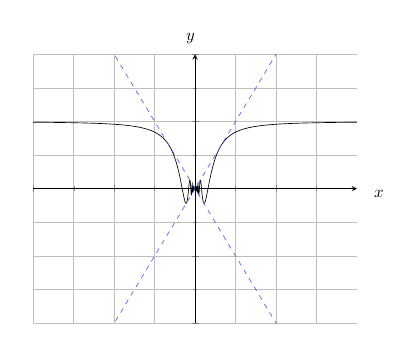
\begin{tikzpicture}[scale=0.60]
 \begin{axis}[grid=both,ymin=-4,ymax=4,xmax=4,xmin=-4,xticklabel=\empty,yticklabel=\empty,
                minor tick num=1,axis lines = middle,xlabel=$x$,ylabel=$y$,label style =
                {at={(ticklabel cs:1.1)}}]
 \addplot[domain = -4:4, samples = 2000, color = black]
 {2*x*sin((1/\x)r)};
 \addplot[dashed, domain = -4:4, samples = 2000, color = RoyalBlue]
 {2*x};
 \addplot[dashed, domain = -4:4, samples = 2000, color = RoyalBlue]
 {-2*x};
     \end{axis}
  \end{tikzpicture}
\end{wrapfigure}

\noindent\exampleblue{ex. $g(x) = 2x \sin(\frac{1}{x})$}
\medskip

$f(x) = -2|x|$, $h(x) = 2|x|$.

$|g(x) = 2|x| < |\sin\frac{1}{x}| < 2x$ for all $x\neq 0$

$|g(x)| \leq h(x) \Rightarrow g(x) \leq h(x)$.\\

and $|g(x)| < -f(x) \Rightarrow g(x) \geq f(x)$.\\

Then, by the squeeze theorem, $\lim_{x\rightarrow 0} g(x) = 0$.
\bigskip
\bigskip


\textit{Proof:} Domain req.: By the hypothesis of the theorem there exists $t>0$ so that $\{ x\in \mathbb{R}, 0< |x-a| <t\} \subset D(g)$.\\

Let $\epsilon>0$. Select $\epsilon_1 = \epsilon/3$, $\epsilon_2 = \epsilon/3$.\\

Since $\lim_{x\rightarrow a} f(x) = L$, there exists $\delta_1 > 0$ so that for all $x\in \mathbb{R}$ with $0 < |x-a| < \delta_1,$ we have $|f(x) - L| < \epsilon_1$.

Similarly, there exists $\delta_2 > 0$ so that for all $x\in \mathbb{R}$ with $0 < |x-a| < \delta_2,$ we have $|f(x) - L| < \epsilon_2$.\\

Let $\delta = $ min($\delta_1, \delta_2, t$), then, for all $x\in \mathbb{R}$ with $0< |x-a| < \delta$, we have:

\begin{align*}
  |g(x) - L| &= |g(x) - f(x) + f(x) -L|\\
             &\leq |g(x) - f(x)| + |f(x) - L|\\
             &\leq |h(x) - f(x)| + |f(x) - L| \text{  for all } x\in (a-t,a) \cup (a, a+t)\\
             &= |h(x) - L + L - f(x)| + |f(x) - L|\\
             &= |h(x) - L| + |L - f(x)| + |f(x) - L|\\
             &= |h(x) - L| + 2|f(x) - L|\\
             &< \epsilon_2 + \epsilon_1 + \epsilon_1 = \epsilon
\end{align*}

\subsection{One-sided Limits}

\redbox{
  Let $f$ be a function and $a \in \mathbb{R}, L\in \mathbb{R}$. We say $\lim_{x \rightarrow a^+} f(x) = L$ if the following holds:
    \begin{itemize}
      \item There exists $t>0$ so that $(a, a+t) \subset D(f)$.
      \item $\forall\; \epsilon>0, \exists\; \delta>0$ s.t. $\forall x\in (a, a+\delta)$, we have $|f(x) - L| < \epsilon$.
    \end{itemize}
}

Similarly, we can define $\lim_{x\rightarrow a^-} f(x) = L$.
\medskip

   \noindent  \redbox{
    Let $f$ be a function and $a \in \mathbb{R}, L\in \mathbb{R}$. We say $\lim_{x \rightarrow a^-} f(x) = L$ if the following holds:
    \begin{itemize}
      \item There exists $t>0$ so that $(a-t, a) \subset D(f)$.
      \item $\forall\; \epsilon>0, \exists\; \delta>0$ s.t. $\forall x\in (a - \delta, a)$, we have $|f(x) - L| < \epsilon$.
    \end{itemize}
}
\bigskip

   \noindent  \redbox{

  \textcolor{red}{\theoremsquare{1}}$$ \lim_{x\rightarrow a}f(x)=L$$ if and only if
  \begin{itemize}
  \item $\lim_{x\rightarrow a^-}f(x)=L$
  \item $\lim_{x\rightarrow a^+}f(x)=L$
  \end{itemize}

}

\subsection{Limits at Infinity}
\redbox{
  Let $f$ be a function and $ L\in \mathbb{R}$. We say $\lim_{x \rightarrow \infty} f(x) = L$ if: \begin{itemize}
    \item There exists $T \in \mathbb{R}$ so that $(T, \infty) \subset D(f)$
    \item For all $\epsilon > 0$, there exists a number $R \in \mathbb{R}$ such that if $x \in \mathbb{R}$ and $x > R$, then $|f(x) - L| < \epsilon$
  \end{itemize}

}
\medskip

Similarly,

\medskip
\noindent\redbox{
  Let $f$ be a function and $ L\in \mathbb{R}$. We say $\lim_{x \rightarrow -\infty} f(x) = L$ if: \begin{itemize}
    \item There exists $T \in \mathbb{R}$ so that $(-\infty, T) \subset D(f)$
    \item For all $\epsilon > 0$, there exists a number $R \in \mathbb{R}$ such that if $x \in \mathbb{R}$ and $x < R$, then $|f(x) - L| < \epsilon$
  \end{itemize}

}

\begin{figure}[h]
\centering
\begin{subfigure}{.5\textwidth}
  \centering
  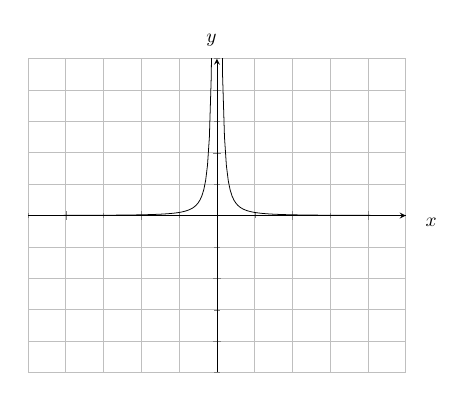
\begin{tikzpicture}[scale = 0.7]

  \begin{axis}[grid=both,ymin=-50,ymax=50,xmax=5,xmin=-5,xticklabel=\empty,yticklabel=\empty,
                 minor tick num=1,axis lines = middle,xlabel=$x$,ylabel=$y$,label style =
                 {at={(ticklabel cs:1.1)}}]
  \addplot[domain = -5:5, samples = 201, color = black]
  {1/x^2};
  \end{axis}
  \end{tikzpicture}
  \caption{$y=\frac{1}{x^2}$}
\end{subfigure}%
\begin{subfigure}{.5\textwidth}
  \centering
  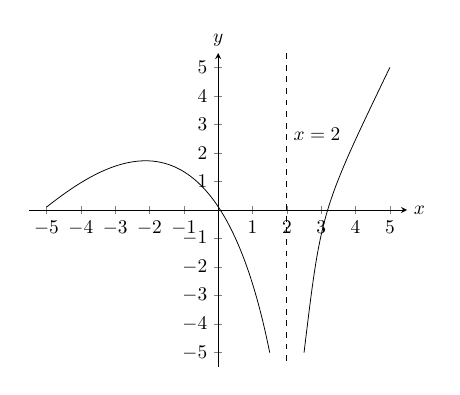
\begin{tikzpicture}[scale = 0.7]
  \begin{axis}[
    axis x line=center,
    axis y line=center,
    xtick={-5,-4,...,5},
    ytick={-5,-4,...,5},
    xlabel={$x$},
    ylabel={$y$},
    xlabel style={at={(1,0.5)},right},
    ylabel style={at={(0.5,1)},above},
    xmin=-5.5,
    xmax=5.5,
    ymin=-5.5,
    ymax=5.5]
    \draw[dashed] (axis cs:2,5.5) -- node[pos=0.3, anchor = south west]{$x=2$}(axis cs:2,-5.5);
    \draw(axis cs:-5,0.1) .. controls(axis cs:-3,2) and (axis cs:0,4) .. (axis cs:1.5,-5);
    \draw(axis cs:2.5,-5) .. controls(axis cs:3,0) .. (axis cs:5,5);
    \end{axis}
    \end{tikzpicture}
  \caption{$y$ approaches $-\infty$  as \newline x approaches 2}
\end{subfigure}
\end{figure}

As seen in figure a) and b), both functions have a limit approaching infinity. We write their limits as $$\lim_{x\rightarrow a}f(x)=(\pm)\infty$$
Thus, we say $x=a$ are their \textbf{asymtotes}.
\bigskip

\noindent \exampleblue{E.x. Let $f(x) = 1/x$, show $\lim_{x\rightarrow \infty} f(x) = 0$}\\

Let $\epsilon >0$, select $R = 1/\epsilon$.

If $x\in (R, \infty)$, then $|f(x) - L| = |f(x)| = |1/x| = 1/x < 1/R = \epsilon$\\
\medskip

\noindent \exampleblue{E.x. $f(x) = \sin(x)$, show for every $L \in \mathbb{R} $, $\lim_{x\rightarrow \infty} f(x) = L$ is false.}\\

\textit{Proof:} Let $L \in \mathbb{R}$,

Since $D(f) = \mathbb{R}$, the domain requirement is met.

Select $\epsilon = 1$. Let $R \in \mathbb{R}$.\\

If $L \leq 0$, select a number $x$ with $x > R$ of the form $x = \frac{\pi}{2} + 2\pi n, n\in \mathbb{Z}$.

Then $f(x) = 1$, so $|f(x) - L| = |1 - L| = 1 - L \geq 1 = \epsilon$.\\

If $L >0$ select a number $x\in \mathbb{R}$ with $x > R$ of the form $x = \frac{3\pi}{2} + 2\pi n, n\in \mathbb{Z}$.

Then $f(x) = -1$, so $|f(x) - L| = |-1 - L| = 1 + L \geq 1 = \epsilon$.

\subsection{Infinite Limits}

\redbox{
  Let $f$ be a function and $a \in \mathbb{R}$. We say $\lim_{x\rightarrow a} f(x) = \infty (-\infty)$, if: \begin{itemize}
    \item Exists $t > 0$ such that $\{ x\in \mathbb{R} : 0 < |x-a| <t\} \subset D(f)$
    \item For all $M \in \mathbb{R}$, exists $\delta > 0$, such that for all $x \in  \mathbb{R}$ with $0 < |x-a| <\delta$, we have $f(x) > M\;\; (f(x) < M)$.
  \end{itemize}
}


\noindent \exampleblue{Ex. $f(x) = \frac{1}{x^2},$ show $\lim_{x\rightarrow 0} f(x) = \infty$.}\\

Since $D(f) = \mathbb{R} \setminus \{ 0\}$, any $t>0$ will work.

Next, let $M\in \mathbb{R}$, select $\delta = \frac{1}{\sqrt{|M|+1}}$.

If $0 < |x-a| < \delta$, $0< |x| <\delta$, then \begin{align*}
      f(x) &= \frac{1}{x^2}\\
           &> \frac{1}{\frac{1}{|M+1|}}\\
           &= |M| + 1 \geq M
\end{align*}

\bigskip
We can also define \reddashedbox{$\lim_{x\rightarrow a^+} f(x) = \infty$, or $\lim_{x\rightarrow a^-} f(x) = \infty$} in the obvious way.
\bigskip

\redbox{
    We say $\lim_{x\rightarrow \infty} f(x) = \infty$ if:\begin{itemize}
      \item $T \in \mathbb{R}$ s.t. $(T, \infty) \subset D(f)$.
      \item For all $M \in \mathbb{R}$, there exists $R \in \mathbb{R}$, such that for all $x\in \mathbb{R}$ with $x> R$, we have $f(x) > M$.
    \end{itemize}
}
\bigskip

We can also define \reddashedbox{$\lim_{x\rightarrow \infty} f(x) = -\infty$} \reddashedbox{$\lim_{x\rightarrow -\infty} f(x) = \infty$}, \reddashedbox{$\lim_{x\rightarrow \infty} f(x) = -\infty$}, \reddashedbox{$\lim_{x\rightarrow -\infty} f(x) = -\infty$} in the obvious way.

\subsection{Existance of Limits}
If $f$ is a function and $a\in \mathbb{R}$ for all $L \in \mathbb{R}$, the statement  ``$\lim_{x\rightarrow a} f(x) = L$'' is false,
then we say $\lim_{x\rightarrow a} f(x)$ does not exist as a real number.\\

If $f$ is a function, $a \in \mathbb{R}$, we say $\lim_{x\rightarrow a} f(x)$ doesn't exist, if for all $L \in \mathbb{R}:$
\[
\begin{cases}
    \lim_{x\rightarrow a}f(x) = L\text{ is false, and}\\
    \lim_{x\rightarrow a}f(x) = \infty\text{ is false, and}\\
    \lim_{x\rightarrow a}f(x) = -\infty\text{ is false}\\
\end{cases}
\]

\subsubsection{Use of product rule}
Despite that limits at infinity are defined as limits that exist, we cannot simply apply the product rules to their product. We need to give individual proof.\\

Example: $\lim_{x\rightarrow a} \frac{1}{(x-a)^2} \cdot \lim_{x\rightarrow a} (x-a)^2$.

\subsection{Asymtotes}
When at least one of the following is true: \newline
$$\lim_{x\rightarrow a}f(x)=\infty,    \lim_{x\rightarrow a^-}f(x)= \infty,   \lim_{x\rightarrow a^+}f(x)= \infty, $$ \newline

$$\lim_{x\rightarrow a}f(x)=-\infty,   \lim_{x\rightarrow a^-}f(x)= -\infty,  \lim_{x\rightarrow a^+}f(x)= -\infty, $$


\redbox{\medskip \centering $x=a$ is a vertical asymtote. \medskip}

\noindent \exampleblue{\textit{Example } Limit of $y=tan(x)$ }

\begin{center}
\begin{figure}[h]
  \centering
  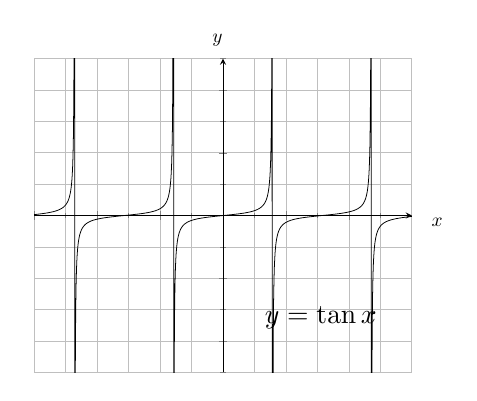
\begin{tikzpicture}[scale = 0.7]
  \begin{axis}[grid=both,ymin=-50,ymax=50,xmax=6,xmin=-6,xticklabel=\empty,yticklabel=\empty,
                 minor tick num=1,axis lines = middle,xlabel=$x$,ylabel=$y$,label style =
                 {at={(ticklabel cs:1.1)}}]
  \addplot[domain = -6:6, samples = 1001, color = black]
  {tan(deg(x))};
  \end{axis}
    \node at(5.2, 1) {$y=\tan x$};
  \end{tikzpicture}
\end{figure}
\end{center}

The vertical asymtotes are:

$$ x = \frac{\pi}{2} + n\pi \:(n\in \mathbb{Z}) $$

\subsection{Limit dependency on Power of Polynomial}

\redbox{
    Let $P$ and $Q$ be non-zero polynomials, of degree $n$ and $m$ respectively, i.e.
    $$ P(x) = a_n x^n + a_{n-1} x^{n-1} + ... + a_0$$
    $$ Q(x) = b_n x^n + b_{n-1} x^{n-1} + ... + b_0$$
    Let $f(x) = \frac{P(x)}{Q(x)}.$\\

    \textcolor{red}{\theoremsquare{1}} If deg P $<$ deg Q $(n<m)$, then $$lim_{x\rightarrow \infty} f(x) = 0$$
    \textcolor{red}{\theoremsquare{2}} If deg P $=$ deg Q $(n=m)$, then $$lim_{x\rightarrow \infty} f(x) = \frac{a_n}{b_m}$$
    \textcolor{red}{\theoremsquare{3}} If deg P $>$ deg Q $(n>m)$, then $$lim_{x\rightarrow \infty} f(x) = \infty \text{ if } \frac{a_n}{b_m} > 0$$
    $$lim_{x\rightarrow \infty} f(x) = -\infty \text{ if } \frac{a_n}{b_m} < 0$$
}

\textit{Proof of 1} To satisfy the domain requirement, we need to ensure $Q(x) \neq 0$. We want to find $T\in R$ so that $Q(x) \neq 0$ for all $x>T$.

We define $B = |b_{m-1}| + |b_{m-2}| + ... + |b_0|$.

If $x\geq 1$, then

\begin{align*}
  |b_{m-1} x^{m-1} + b_{m-2} x^{m-2} + ... b_0| &\leq |b_{m-1} x^{m-1}| + |b_{m-2} x^{m-2}| +...+ |b_0|\\
                                                &\leq |b_{m-1}||x^{m-1}| + |b_{m-2}||x^{m-1}| +...+ |b_0||x^{m-1}|\\
                                                &\leq B|x^{m-1}|
\end{align*}

Thus, we conclude if $x\geq 1$,

$$ a - |b| \leq a+b \leq a + |b|$$
$$ \Downarrow $$
$$b_m x^m - Bx^{m-1} \leq Q(x) \leq b_mx^m + Bx^{m-1}$$

Next, we take
$$ b_mx^m - Bx^{m-1} = x^{m-1}(b_m x - B)$$

And let $T = B/|b_m|$.

If $x > T$, then\\

\noindent If $b_m < 0$,\\
Since $B>0$, $b_mx<0, b_mx-B < 0$.\\
Also $x^{m-1} > 0$, thus $x^{m-1}(b_m x -B) < 0$.\\
$Q(x) \neq 0$.\\

\noindent If $b_m > 0$,\\
$b_mx-B > 0$.\\
Also $x^{m-1} > 0$, thus $x^{m-1}(b_m x -B) > 0$.\\
$Q(x) \neq 0$.\\

\noindent Thus, $T = B/|b_m|$ will work.\\
Next, let $\epsilon > 0$.\\
We need to find $R \in \mathbb{R}$, so that for all $x > R$, $|\frac{P(x)}{Q(x)}| < \epsilon$.\\

Similar to $B$, we define $C = |a_{n-1}| + |a_{n-2}| + ... + |a_0|$. Then if $x \geq 1$, $$|P(x)| \leq Cx^n$$

Next, if we choose $x > 2B/|b_m|$, then
\begin{align*}
  x^{m-1}(|b_m|x - 2B) &> 0\\
  |b_m| x^m - 2B x^{m-1} &> 0\\
  \frac{1}{2} |b_m| x^m &> B x^{m-1}\\
  - \frac{1}{2} |b_m| x^m &< -B x^{m-1} \Rightarrow \text{ add to both sides } |b_m|x^m\\
  \frac{1}{2} |b_m| x^m &< |b_m| x^m -B x^{m-1}< Q(x)
\end{align*}

Select $R =$ max($1, 2B/b_m, 2C/|b_m|\epsilon$), then:\\
\begin{align*}
  \frac{|P(x)|}{|Q(x)|} \leq \frac{Cx^n}{\frac{1}{2}|b_m|x^m} &= \frac{2C}{|b_m|} \cdot \frac{1}{x^{n-m}}\\
                                                  &\leq \frac{2C}{|b_m|}\cdot \frac{1}{x}\; \text{  Since   } n-m \geq 1, 1/x \geq x\\
                                                  &< \frac{2C}{|b_m|} \cdot \frac{1}{R}\\
                                                  &< \frac{2C}{|b_m|} \cdot \frac{|b_m|\epsilon}{2C} = \epsilon
\end{align*}

\medskip

\textit{Proof of 2:} Suppose \[
  \begin{rcases*}
      P(x) = a_nx^n + ... + a_0 \\
      Q(x) = b_mx^n + ... + a_0
  \end{rcases*} \text{ to some degree }\]

\noindent First, $$\lim_{x\rightarrow \infty} \frac{a_n}{b_n} = \frac{a_n}{b_n}$$
Next, $$\frac{P(x)}{Q(x)} - \frac{a_n}{b_n} = \frac{b_nP(x) - a_n Q(x)}{b_nQ(x)}$$ when $Q(x) \neq 0$.

\begin{align*}
  &= \frac{b_n(a_n x^n + a_{n-1} x^{n-1} + ... +a_0) - a_n (b_n x^n + b_{n-1} x^{n-1} + ... +b_0)}{b_n Q(x)}\\
  &= \frac{b_n a_n x^n - b_n a_n x^n + b_n(a_{n-1} x^{n-1} + ... +a_0) - a_n(b_{n-1} x^{n-1} + ... +b_0) }{b_n Q(x)}\\
  &= \frac{S(x)}{b_n Q(x)} \text{  Where deg. of S is less than deg. of Q}
\end{align*}

So $$\lim_{x\rightarrow \infty} (\frac{P(x)}{Q(x)} - \frac{a_n}{b_n}) = \lim_{x\rightarrow \infty} \frac{S(x)}{b_n Q(x)} = 0$$

Then $$\lim_{x\rightarrow \infty} \frac{P(x)}{Q(x)} = \lim_{x\rightarrow \infty} (\frac{P(x)}{Q(x)} - \frac{a_n}{b_n} + \frac{a_n}{b_n}) = 0 + \frac{a_n}{b_n} = \frac{a_n}{b_n}$$

\medskip

\textit{Proof of 3:} To satisfy the domain requirement, we need to ensure $Q(x) \neq 0$. We want to find $T\in R$ so that $Q(x) \neq 0$ for all $x>T$.

We define $B = |b_{m-1}| + |b_{m-2}| + ... + |b_0|$.

If $x\geq 1$, then
\begin{align*}
  |b_{m-1} x^{m-1} + b_{m-2} x^{m-2} + ... b_0| &\leq |b_{m-1} x^{m-1}| + |b_{m-2} x^{m-2}| +... |b_0|\\
                                                &\leq |b_{m-1}||x^{m-1}| + |b_{m-2}||x^{m-1}| +... |b_0||x^{m-1}|\\
                                                &\leq B|x^{m-1}|
\end{align*}

We can satisfy the domain requirement similar to proof 1.

Next, let $M \in \mathbb{R}$.

We need to find $R\in \mathbb{R}$, so that for all $x > R$, $ P(x)/Q(x) > M$.\\

We can assume $a_n > 0, b_n > 0$, and that $n > m$

Similar to $B$, we define $A = |a_{n-1}| + |a_{n-2}| + ... + |a_0|$. We have:

$$a_n x^n - Ax^{n-1} \leq P(x) \leq a_nx^n + Ax^{n-1}$$

Next, if we choose $x > 2A/a_n$, then

\begin{align*}
  x^{n-1}(a_n x - 2A) &> 0\\
  a_n x^n - 2A x^{n-1} &> 0\\
  \frac{1}{2} a_n x^n &> A x^{n-1}\\
  - \frac{1}{2} a_n x^n &< -A x^{n-1}\\
  \frac{1}{2} a_n x^n &< a_n x^n -A x^{n-1}< P(x)
\end{align*}

We define $C = B + b_m$. If $x\geq 1$,
$$ Q(x) \leq Bx^m + b_m x^m$$
$$ Q(x) \leq Cx^m$$

We can define $M' = $ max($1,M$), so that $M' \geq M$.

Select $R = $ max($1, \; 2A/a_n, \; 2Ca_nM'$)
\medskip

Let $x>R$.
Since $\frac{1}{2} a_n x^n < P(x)$,
$Q(x) \leq Cx^m$
\begin{align*}
  \frac{P(x)}{Q(x)} > \frac{1/2 |a_n|x^n}{Cx^m} &= \frac{1}{2C|a_n|} \cdot x^{n-m}\\
                                                  &\geq \frac{1}{2C|a_n|} \cdot x \;\; \text{  Since   } n-m \geq 1, 1/x \leq x\\                               &\geq \frac{1}{2C|a_n|} \cdot M'\\
                                                  &> \frac{1}{2C|a_n|} \cdot 2C|a_n|M = M
\end{align*}

For $a_n < 0$ and $b_m < 0$, the proof is similar where $ P(x)/Q(x) > M$;\\

For $a_n > 0$ and $b_m < 0$, or $a_n < 0$ and $b_m >0$, the proof is different as $ P(x)/Q(x) < M$.

\subsection{Limit Laws}
*Suppose $c$ is a constant and $\lim_{x\rightarrow a} f(x)$ and $\lim_{x\rightarrow a} g(x)$ exists,
\medskip

\redbox{
\begin{spreadlines}{20pt}
\begin{gather}
\lim_{x\rightarrow a} [f(x)+g(x)] = \lim_{x\rightarrow a} f(x) + \lim_{x\rightarrow a} g(x) \\
\lim_{x\rightarrow a} [f(x)-g(x)] = \lim_{x\rightarrow a} f(x) - \lim_{x\rightarrow a} g(x) \\
\lim_{x\rightarrow a} [cf(x)] = c\lim_{x\rightarrow a} f(x)\\
\lim_{x\rightarrow a} [f(x)g(x)] = \lim_{x\rightarrow a} f(x) \cdot \lim_{x\rightarrow a} g(x) \\
\lim_{x\rightarrow a} \frac{[f(x)]}{[g(x)]} = \frac{\lim_{x\rightarrow a} f(x)} {\lim_{x\rightarrow a} g(x)}  \:(\lim_{x\rightarrow a} g(x)\neq 0)
\end{gather}
\end{spreadlines}}

\redbox{
  \centering
  $$\lim_{x\rightarrow a} [f(x)]^n = [\lim_{x\rightarrow a}f(x)]^n$$ \newline
  $$\lim_{x\rightarrow a} \sqrt[n]{f(x)} = \sqrt[n]{\lim_{x\rightarrow a} f(x)}$$
}

\subsection{Limit Calculations}
\noindent\exampleblue{\textit{Example 1.}
       Find $\lim_{h\rightarrow 0} \frac{(3+h)^2-9}{h}$
}

\begin{align*}
  F(h) &= \frac{(3+h)^2-9}{h}\\
       &= \frac{h^2+6h+9-9}{h}\\
       &= h+6
\end{align*}
By evaluation, $\lim_{h\rightarrow 0} h+6 = 6$


\subsubsection{Direct Substitution Property}

\hspace{1cm} If $f$ is a \textbf{polynomial} or a \textbf{rational function} and $a$ is in the domain of $f$, then:\newline
\redbox{\centering $$\lim_{x\rightarrow a} f(x) = f(a)$$}
\medskip

\noindent\exampleblue{\textit{Example 2.}
       Find $\lim_{t\rightarrow 0} \frac{\sqrt{t^2+9}-3}{t^2}$
}

\begin{align*}
       &= \lim_{t\rightarrow 0} \frac{\sqrt{t^2+9}-3}{t^2} \cdot \frac{\sqrt{t^2+9}+3}{\sqrt{t^2+9}+3}\\
       &= \lim_{t\rightarrow 0} \frac{t^2+9-9}{t^2(\sqrt{t^2+9}+3)}\\
       &= \lim_{t\rightarrow 0} \frac{t^2}{t^2\sqrt{t^2+9}+3t^2}\\
       &= \lim_{t\rightarrow 0} \frac{1}{\sqrt{t^2+9}+3}\\
       &= \frac{1}{\sqrt{\lim_{t\rightarrow 0} t^2 +9} +3}\\
       & = \frac{1}{\sqrt{9}+3} = \frac{1}{6}
\end{align*}

\noindent\exampleblue{\textit{Example 3.}
       Find $\lim_{x\rightarrow 1} \frac{\sqrt[3]{x}-1}{\sqrt{x}-1}$
}

\section{Continuity}

\redbox{
    Let $f$ be a function, and let $a \in \mathbb{R}$. We say that $f$ is continuous at $a$, if
    $$\lim_{x\rightarrow a} f(x) = f(a)$$
}

In particular, this implies:
\begin{enumerate}[label=\protect\circled{\arabic*}]
  \item $a \in D(f)$
  \item $f(a) \in \mathbb{R}$
  \item $\lim_{x\rightarrow a} f(x)$ exists as a real number
\end{enumerate}
\medskip

Ex.\[
f(x)= \begin{cases}
    x \text{ , if } x\in \mathbb{Q}\\
    0 \text{ , if } x\notin \mathbb{Q}\\
\end{cases}
\]

$\lim_{x\rightarrow 0} f(x) = 0 = f(0)$.

So $f$ is continuous at $0$. It is not continuous at every other point. If f is not continuous at $a$, we say it is \textbf{discontinuous} at $a$.
\medskip

\redbox
{
   If $\lim_{x\rightarrow a^+} f(x) = f(a)$, we say $f$ is right continuous.

   If $\lim_{x\rightarrow a^-} f(x) = f(a)$, we say $f$ is left continuous.
}
\medskip

\redbox
{
    Let $f$ be a function, and let $(a,b)$ be an (open) interval. We say $f$ is continuous on $(a,b)$ if it is continuous at every point $x\in \mathbb{R}, x\in (a,b)$.
}
\medskip

\redbox
{
      If $f$ is a function , and $[a,b]$ is a closed interval, We say $f$ is continuous on $[a,b]$ if \begin{itemize}
        \item $\lim_{x\rightarrow c} f(x) = f(c)$ for all $c\in (a,b)$.
        \item $\lim_{x\rightarrow a^+} f(x) = f(a)$
        \item $\lim_{x\rightarrow b^-} f(x) = f(b)$
      \end{itemize}
}

\noindent \textit{Lemma 1}:

Let $f$ be a function that is continuous at the point $c \in \mathbb{R}$.

If $f(c) \neq 0$, then there exists $\delta >0$, so that $f(x)$ is defined, and $f(x) \neq 0$ for all $$x \in (c-\delta, c+\delta)$$

Ex. \[
f(x)= \begin{cases}
    1 \text{ , if } x\in \mathbb{Q}\\
    x \text{ , if } x\notin \mathbb{Q}\\
\end{cases}
\]

\noindent\textit{Proof of Lemma:}

Since $f$ is continuous at $c$, $\lim_{x\rightarrow c} f(x) = f(c) \neq 0$.

Choose $\epsilon = \frac{|f(c)|}{2}$\\

Then, there exists $\delta > 0$, so that for every $x\in \mathbb{R}$ with $0< |x-c| <\delta$, $f(x)$ exists and $|f(x) - f(c)| < \epsilon$.

\end{document}
